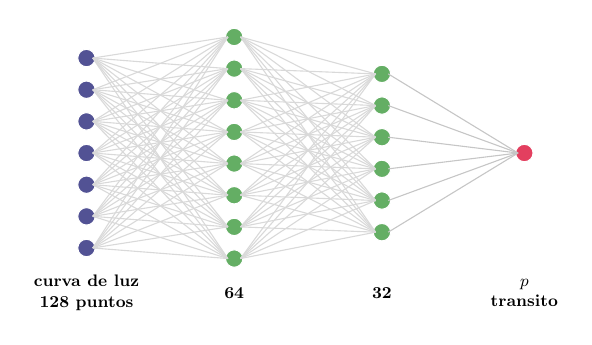
\begin{tikzpicture}[scale=0.67,transform shape]
\def\xA{0} \def\xB{2.8} \def\xC{5.6} \def\xD{8.3}
\foreach \y in {-1.8,-1.2,-0.6,0,0.6,1.2,1.8} {\node[circle,fill=MidnightBlue!75,draw=white,minimum size=7pt] at (\xA,\y) {};}
\foreach \y in {-2.0,-1.4,-0.8,-0.2,0.4,1.0,1.6,2.2} {\node[circle,fill=ForestGreen!70,draw=white,minimum size=7pt] at (\xB,\y) {};}
\foreach \y in {-1.5,-0.9,-0.3,0.3,0.9,1.5} {\node[circle,fill=ForestGreen!70,draw=white,minimum size=7pt] at (\xC,\y) {};}
\node[circle,fill=Crimson!82,draw=white,minimum size=9pt] at (\xD,0) {};
\foreach \ya in {-1.8,-1.2,-0.6,0,0.6,1.2,1.8} {\foreach \yb in {-2.0,-1.4,-0.8,-0.2,0.4,1.0,1.6,2.2} {\draw[gray!30,thin] (\xA+0.12,\ya)--(\xB-0.12,\yb);}}
\foreach \ya in {-2.0,-1.4,-0.8,-0.2,0.4,1.0,1.6,2.2} {\foreach \yb in {-1.5,-0.9,-0.3,0.3,0.9,1.5} {\draw[gray!30,thin] (\xB+0.12,\ya)--(\xC-0.12,\yb);}}
\foreach \ya in {-1.5,-0.9,-0.3,0.3,0.9,1.5} {\draw[gray!45,thin] (\xC+0.12,\ya)--(\xD-0.12,0);}
\node[font=\small\bfseries,align=center] at (\xA,-2.65) {curva de luz\\128 puntos};
\node[font=\small\bfseries] at (\xB,-2.65) {64};
\node[font=\small\bfseries] at (\xC,-2.65) {32};
\node[font=\small\bfseries,align=center] at (\xD,-2.65) {$p$\\transito};
\end{tikzpicture}
